\documentclass[11pt]{scrartcl}
\usepackage[T1]{fontenc}
\usepackage[a4paper, left=3cm, right=2cm, top=2cm, bottom=2cm]{geometry}
\usepackage[activate]{pdfcprot}
\usepackage[ngerman]{babel}
\usepackage[parfill]{parskip}
\usepackage[utf8]{inputenc}
\usepackage{kurier}
\usepackage{amsmath}
\usepackage{amssymb}
\usepackage{xcolor}
\usepackage{epstopdf}
\usepackage{txfonts}
\usepackage{fancyhdr}
\usepackage{graphicx}
\usepackage{prettyref}
\usepackage{hyperref}
\usepackage{eurosym}
\usepackage{setspace}
\usepackage{units}
\usepackage{eso-pic,graphicx}
\usepackage{icomma}
\usepackage{pdfpages}

\definecolor{darkblue}{rgb}{0,0,.5}
\hypersetup{pdftex=true, colorlinks=true, breaklinks=false, linkcolor=black, menucolor=black, pagecolor=black, urlcolor=darkblue}



\setlength{\columnsep}{2cm}


\newcommand{\arcsinh}{\mathrm{arcsinh}}
\newcommand{\asinh}{\mathrm{arcsinh}}
\newcommand{\ergebnis}{\textcolor{red}{\mathrm{Ergebnis}}}
\newcommand{\fehlt}{\textcolor{red}{Hier fehlen noch Inhalte.}}
\newcommand{\betanotice}{\textcolor{red}{Diese Aufgaben sind noch nicht in der Übung kontrolliert worden. Es sind lediglich meine Überlegungen und Lösungsansätze zu den Aufgaben. Es können Fehler enthalten sein!!! Das Dokument wird fortwährend aktualisiert und erst wenn das \textcolor{black}{beta} aus dem Dateinamen verschwindet ist es endgültig.}}
\newcommand{\half}{\frac{1}{2}}
\renewcommand{\d}{\, \mathrm d}
\newcommand{\punkte}{\textcolor{white}{xxxxx}}
\newcommand{\p}{\, \partial}
\newcommand{\dd}[1]{\item[#1] \hfill \\}

\renewcommand{\familydefault}{\sfdefault}
\renewcommand\thesection{}
\renewcommand\thesubsection{}
\renewcommand\thesubsubsection{}


\newcommand{\themodul}{Halbleiter und Nanotechnologie}
\newcommand{\thetutor}{Prof. Förster}
\newcommand{\theuebung}{Übung 3}

\pagestyle{fancy}
\fancyhead[L]{\footnotesize{C. Hansen}}
\chead{\thepage}
\rhead{}
\lfoot{}
\cfoot{}
\rfoot{}

\title{\themodul{}, \theuebung{}, \thetutor}


\author{Christoph Hansen \\ {\small \href{mailto:chris@university-material.de}{chris@university-material.de}} }

\date{}


\begin{document}

\maketitle

Dieser Text ist unter dieser \href{http://creativecommons.org/licenses/by-nc-sa/4.0/}{Creative Commons} Lizenz veröffentlicht.

\textcolor{red}{Ich erhebe keinen Anspruch auf Vollständigkeit oder Richtigkeit. Falls ihr Fehler findet oder etwas fehlt, dann meldet euch bitte über den Emailkontakt.}

\tableofcontents


\newpage



\section{Aufgabe 1}

\subsection*{a)}

Der Leitwert ist auch der Volumenfluss $q_V = C$, also:

\begin{align*}
C_{H_2} &= \sqrt{\frac{RT}{2 \pi M}} \cdot A = \sqrt{\frac{8,31 \cdot 300}{2 \pi \cdot 2 \cdot 10^{-3}}} \cdot \frac{\pi \cdot \left( 0,3 \cdot 10^{-6} \right)^2}{4} = \unit[3,14 \cdot 10^{-11}]{m^3/s} \\
C_{N_2} &= \sqrt{\frac{RT}{2 \pi M}} \cdot A = \sqrt{\frac{8,31 \cdot 300}{2 \pi \cdot 28 \cdot 10^{-3}}} \cdot \frac{\pi \cdot \left( 0,3 \cdot 10^{-6} \right)^2}{4} = \unit[8,4 \cdot 10^{-12}]{m^3/s}
\end{align*}


\subsection*{b)}

Die Leckraten sind:

\begin{align*}
L_{H_2} &= P_a \cdot q_V = 0,5 \cdot 10^5 \cdot 3,14 \cdot 10^{-11} = \unit[1,5 \cdot 10^{-6}]{Pa \ m^3 /s} \\
L_{N_2} &= 0,5 \cdot 10^5 \cdot 8,4 \cdot 10^{-12} = \unit[2,5 \cdot 10^{-7}]{Pa \ m^3 /s}
\end{align*}


\subsection*{c)}


Wir haben einen linearen Druckanstieg. $I_E$ ist der einlaufende Gasstrom also die Leckrate:

\begin{align*}
P &= P_0 + \frac{I_E}{V_r} \cdot t \\
P_{H_2} &= \frac{1,5 \cdot 10^{-8}}{0,3} \cdot 600 = \unit[3 \cdot 10^{-5}]{mbar} \\
P_{H_2} &= \frac{2,5 \cdot 10^{-9}}{0,3} \cdot 600 = \unit[5 \cdot 10^{-6}]{mbar} \\
\hfil \\
P_{ges} &= P_0 + P_{N_2} + P_{H_2} = \unit[3,5 \cdot 10^{-5}]{mbar}
\end{align*}


\subsection*{d)}

Aus den Enddrücken von Wasserstoff und Stickstoff berechnen wir den Gesamtenddruck:

\begin{align*}
P_{e,H_2} &= \frac{P_a \cdot C}{S} = \frac{0,5 \cdot 10^5 \cdot 3,1 \cdot 10^{-11}}{0,2} = \unit[7,75 \cdot 10^{-6}]{Pa} \\
P_{e,N_2} &= \frac{P_a \cdot C}{S} = \frac{0,5 \cdot 10^5 \cdot 8,9 \cdot 10^{-12}}{0,2} = \unit[1,26 \cdot 10^{-6}]{Pa} \\
\hfil \\
P_{ges} &= P_{e,H_2} + P_{e,N_2} = \unit[9 \cdot 10^{-6}]{Pa}
\end{align*}



\section{Aufgabe 2}

\subsection*{a)}

Der Leitwert des Rohres ist:

\begin{align*}
C_L &= 1,2 \cdot \sqrt{\frac{T}{M}} \cdot \frac{D^3}{L} = 1,2 \cdot \sqrt{\frac{300}{28 \cdot 10^{-3}}} \cdot \frac{\left( 50 \cdot 10^{-3} \right)^3}{5} = \unit[3,1 \cdot 10^{-3}]{m^3/s} = \unit[3,1]{l/s}
\intertext{Den Klausingfaktor müssen wir nicht berücksichtigen, das das Verhältnis vonm Länge zu Durchmesser sehr groß ist.}
\end{align*}


\subsection*{b)}

\begin{align*}
\frac{1}{S_{eff}} &= \frac{1}{C_V} + \frac{1}{C_L} + \frac{1}{S_P} = \frac{1}{10} + \frac{1}{3,1} + \frac{1}{200} = \unit[0,43]{s/l} \\
\Leftrightarrow S_{eff} &= \unit[2,2]{l/s}
\end{align*}


\section{Aufgabe 3}

Das Rohr ist $\unit[3]{m}$ lang!


\subsection*{a)}

Die Knudsenzahl lässt sich so bestimmen:

\begin{align*}
K &= \frac{\lambda}{D} \qquad \text{mit} \qquad \lambda = \frac{\lambda_P}{\bar{P}} \\
&= \frac{\frac{\lambda_P}{\frac{P_1 + P_2}{2}}}{D} = \frac{\frac{79 \cdot 10^{-6}}{275}}{15 \cdot 10^{-3}} = 1,9 \cdot 10^{-3} < 10^{-2}
\end{align*}

Es handelt sich um eine reibungsbehaftete Strömung.


\subsection*{b)}

\begin{align*}
C_{Rohr} &= 2,454 \cdot 10^{-2} \cdot \frac{D^4}{\eta l} \cdot \bar{P} = 2,454 \cdot 10^{-2} \cdot \frac{\left( 1,5 \cdot 10^{-3} \right)^4 \cdot 275}{0,0086 \cdot 10^{-3} \cdot 3} = \unit[1,32 \cdot 10^{-2}]{m^3/s}
\end{align*}


\subsection*{c)}

\begin{align*}
I &= C \cdot \Delta P = 1,32 \cdot 10^{-2} \cdot \left( 300 - 250 \right) = \unit[6,6 \cdot 10^{-1}]{Pa \ m^3 / s}
\end{align*}



\section{Aufgabe 4}

\subsection*{a)}

Wir müssen die Formel für die Energie zweifach nach $k$ ableiten:

\begin{align*}
\frac{\p E}{\p k} &= 2 \cdot 9,13 \cdot 10^{-38} \cdot \left( k - k_0 \right) \\
\frac{\p^2 E}{\p^2 k} &= 2 \cdot 9,13 \cdot 10^{-38} 
\intertext{Nun müssel wir noch die masseabhängige Energieformel ableiten:}
E &= \frac{\hbar^2 \cdot k^2}{2m} \\
\frac{\p E}{\p k} &= \frac{\hbar^2 \cdot k}{m} \\
\frac{\p^2 E}{\p^2 k} &= \frac{\hbar^2}{m^*}
\intertext{Nun können wir gleichsetzen:}
\Leftrightarrow \frac{1}{m^*} &= \frac{\p^2 E}{\p^2 k} \cdot \frac{1}{\hbar^2} = \frac{2 \cdot 9,13 \cdot 10^{-38}}{\left( 1,054 \cdot 10^{-34} \right)^2} = 1,6 \cdot 10^{31} \\
\Leftrightarrow m^* &= \unit[6,08 \cdot 10^{-32}]{kg} \\
\Rightarrow \frac{m^*}{m_e} &= \frac{6,08 \cdot 10^{-32}}{9,1 \cdot 10^{-31}} = 0,067
\end{align*}


\subsection*{b)}


\begin{figure}[h]
	\centering
	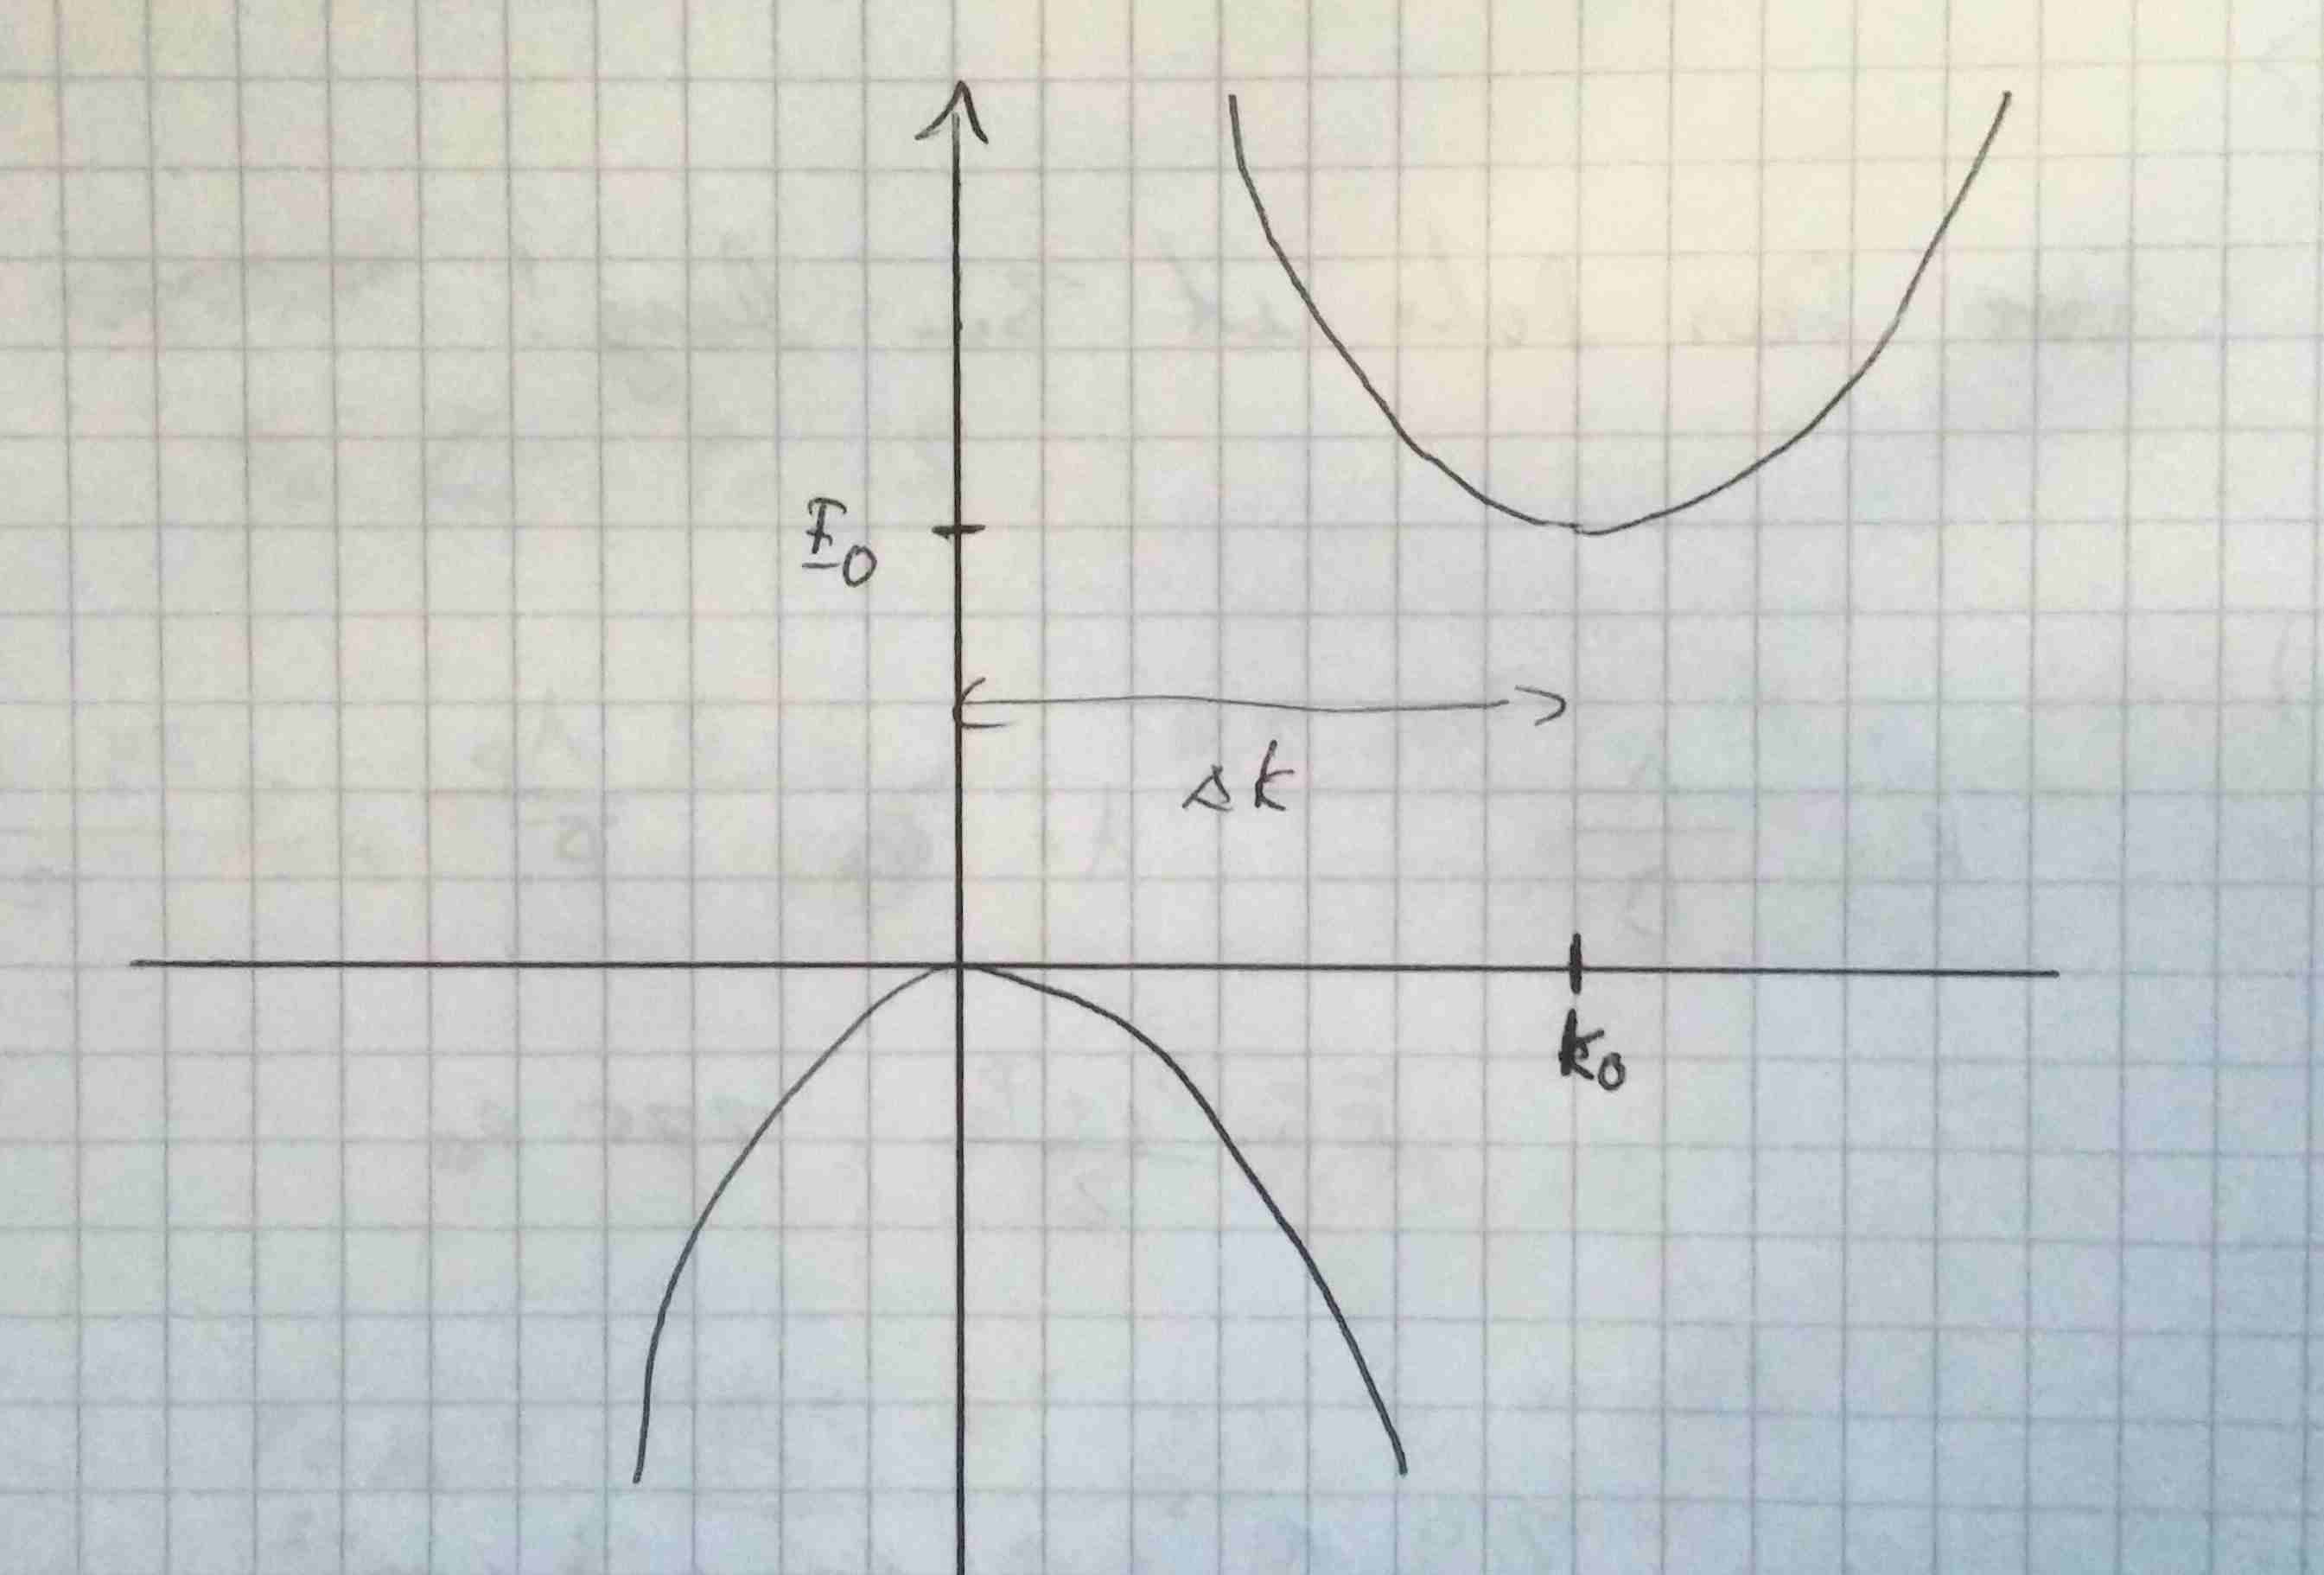
\includegraphics[scale=0.1]{A4_1.jpg}
\end{figure}

Es ist ein indirekter Halbleiter, das es den Versatz $\Delta k$ gibt.



\subsection*{c)}

\begin{align*}
n &= N_c \cdot e^{- \frac{E_L - E_F}{kT}} \\
\Leftrightarrow \frac{n}{N_c} &= e^{- \frac{\Delta E}{kT}} \\
\Leftrightarrow \frac{\Delta E}{kT} &= \ln \left( \frac{n}{N_c} \right) = \ln \left( \frac{10^{23}}{4,35 \cdot 10^{23}} \right) = 1,47
\intertext{Wir rechnen mit $kT = \unit[26]{meV}$}
\Leftrightarrow \Delta E &= 1,47 \cdot 26 = \unit[38,2]{meV}
\end{align*}



\section{Aufgabe 5}

\subsection*{a)}

\begin{figure}[h]
	\centering
	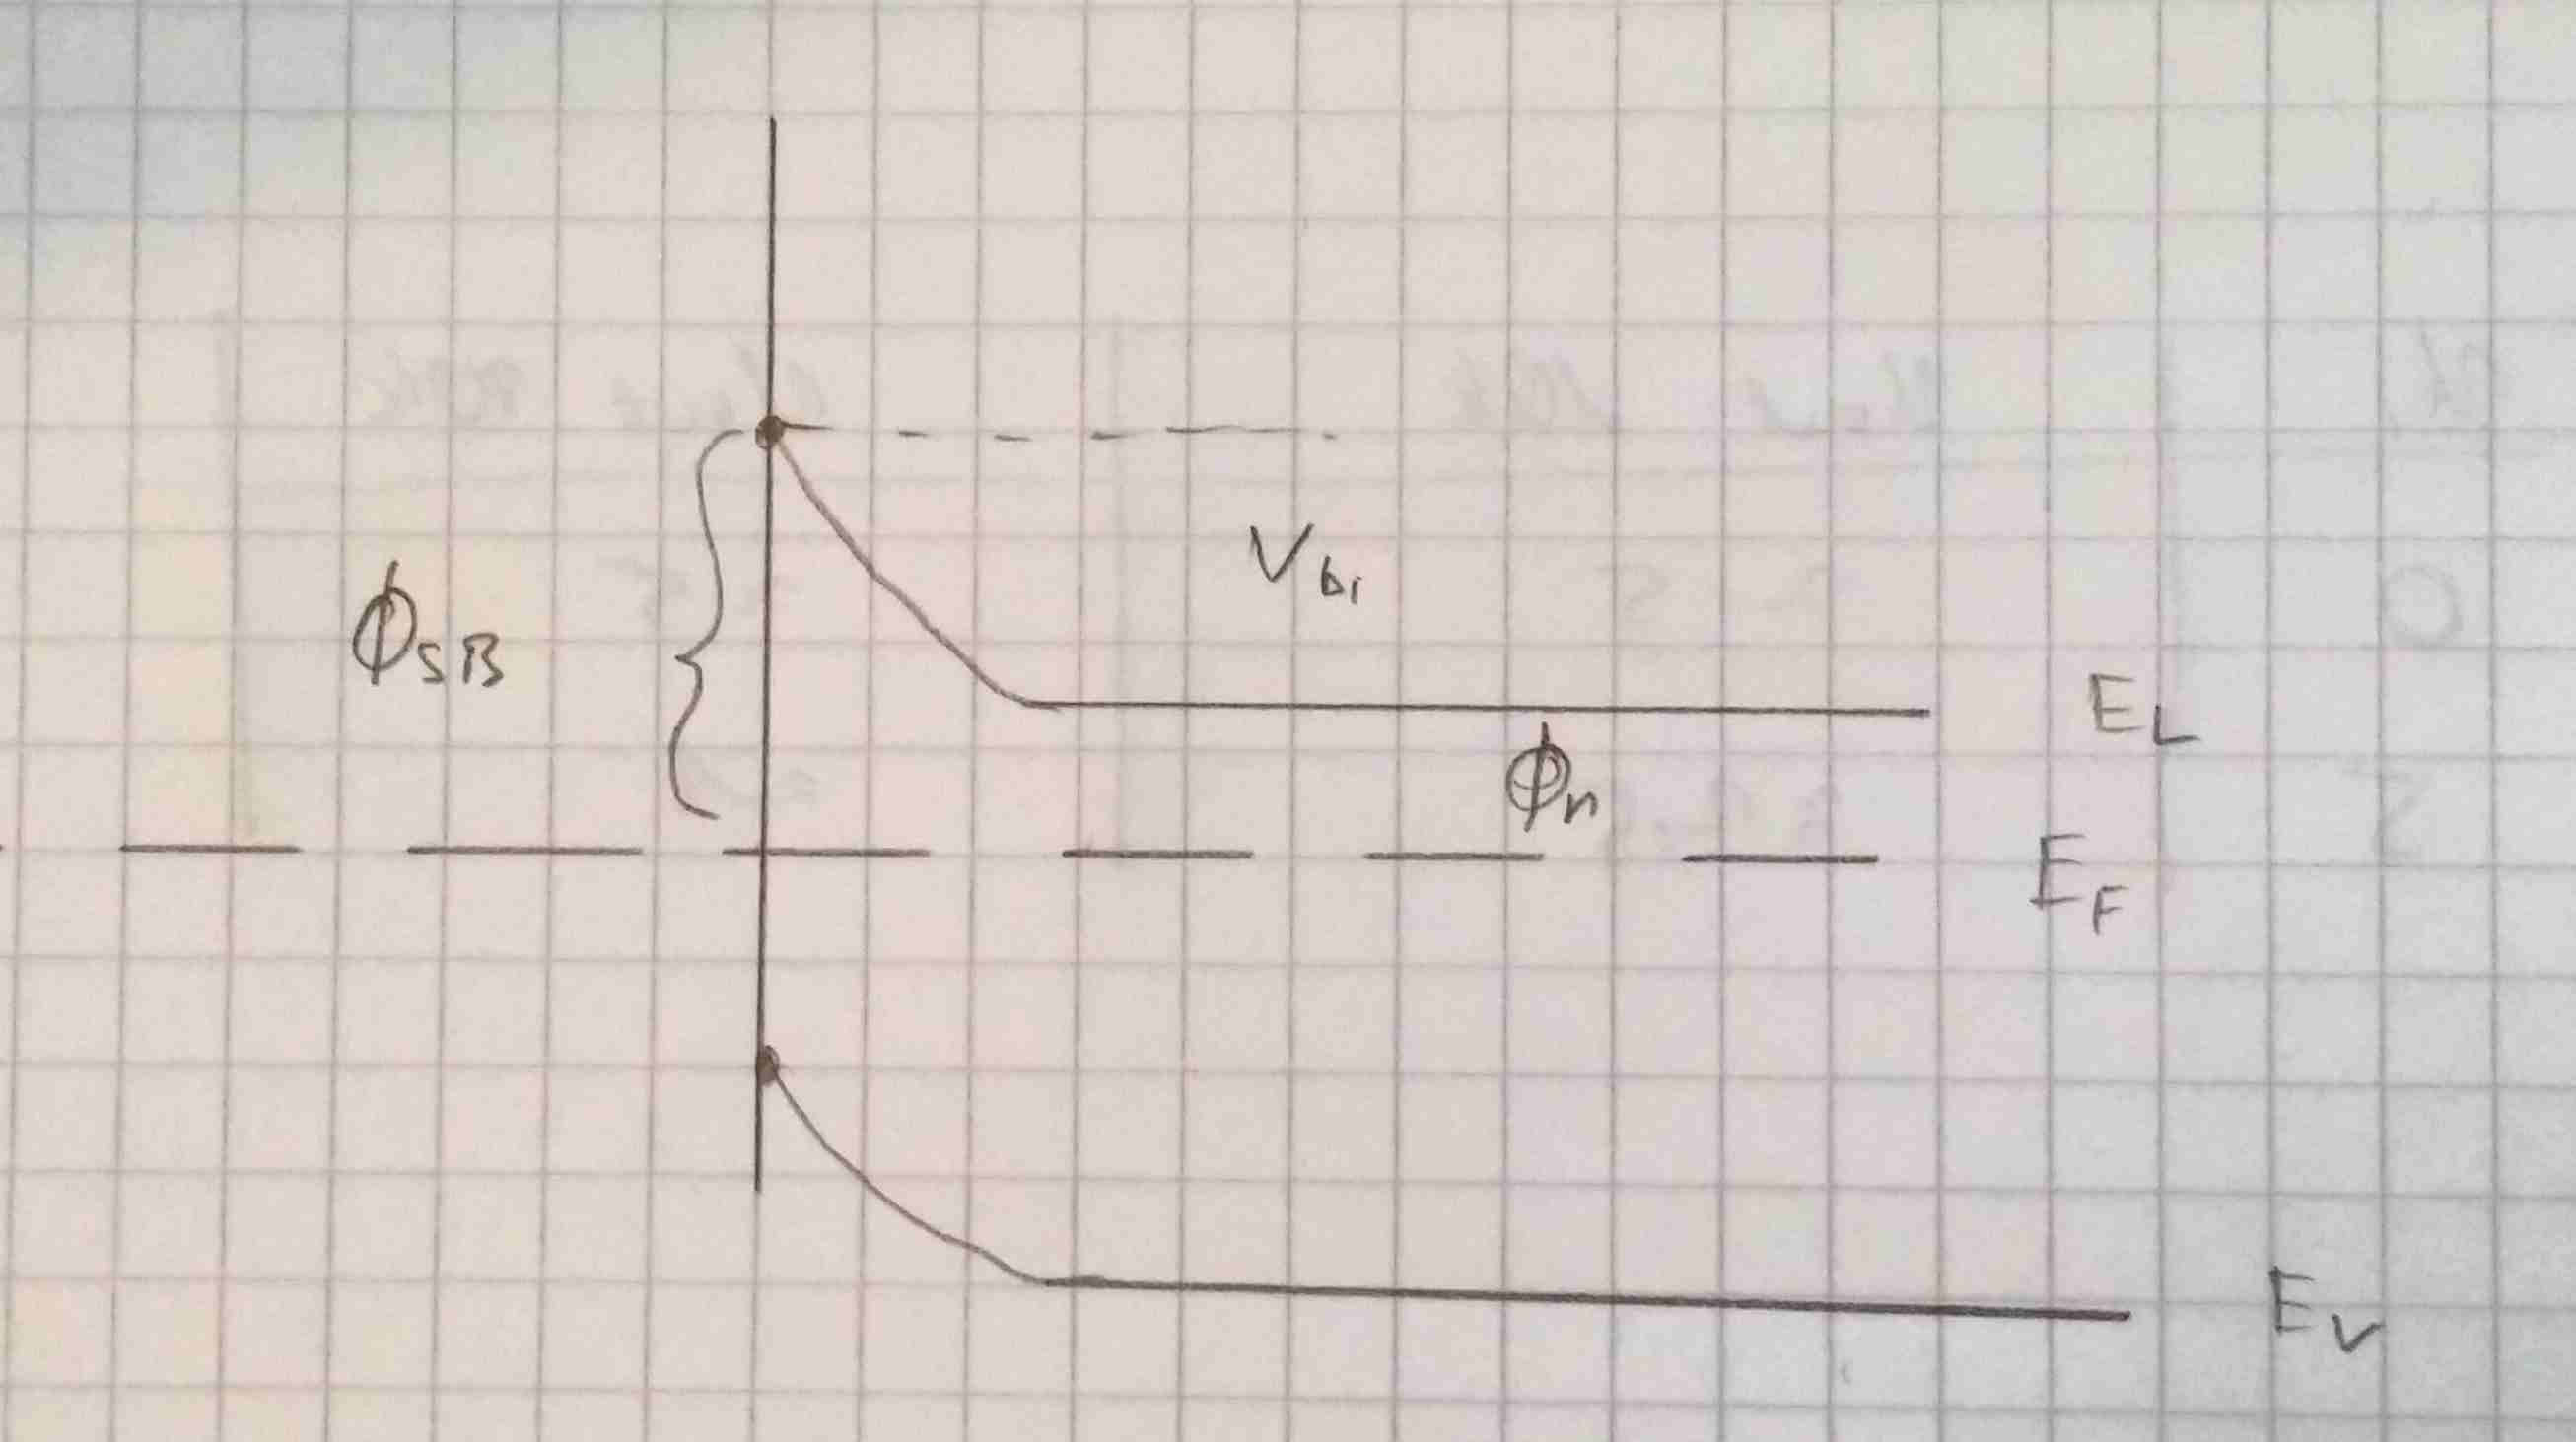
\includegraphics[scale=0.16]{A5_1.jpg}
\end{figure}



\subsection*{b)}

\begin{align*}
\phi_{SB} &= V_{bi} + \phi_n \\
\Leftrightarrow V_{bi} &= \phi_{SB} - \phi_n = 0,65 - 0,09 = \unit[0,56]{V}
\end{align*}


\subsection*{c)}

\begin{align*}
w &= \sqrt{\frac{2 \epsilon_r \epsilon_0 \cdot \left( V_{bi} + V_R \right)}{e \cdot N_d}} = \sqrt{\frac{2 \epsilon_r \epsilon_0 \cdot 0,56}{1,6 \cdot 10^{-19} \cdot 1,6 \cdot 10^{22}}} = \unit[220]{nm}
\end{align*}


\subsection*{d)}

\begin{align*}
C' &= \frac{\epsilon_r \cdot \epsilon_0}{w} = \frac{8,85 \cdot 10^{-12} \cdot 12,9}{220 \cdot 10^{-9}} = \unit[5,1 \cdot 10^{-4}]{F/m}
\end{align*}


\section{Aufgabe 6}


Wir müssen jeweils zwei Lastgeraden berechnen. Diese gehen laufen von $\unit[5]{V}$ auf der x-Achse zu dem berechneten Strom auf der y-Achse:

\begin{align*}
I_{10k} &= \frac{U_B}{R_L} = \frac{5}{10000} = \unit[0,5]{mA} \\
I_{20k} &= \frac{U_B}{R_L} = \frac{5}{20000} = \unit[0,25]{mA}
\end{align*}



\subsection*{b)}

\begin{center}
	\begin{tabular}{c|c|c}
	$U_i$	& $U_{out}$ 10k & $U_{out}$ 20k \\ 
		\hline  
	0	& 5 & 5 \\ 
		\hline 
	5	& 2,5 & 1 \\ 
	\end{tabular} 
\end{center}


Man würde den $\unit[20]{k \Omega}$ Widerstand nehmen, da dieser mehr schwankt.















\end{document}